\documentclass[aspectratio=169,11pt]{beamer}
\usetheme{Madrid}
\usecolortheme{seahorse}
\usepackage{amsmath,amssymb}
\usepackage{tikz}
\usetikzlibrary{arrows.meta,positioning,shapes.geometric}
\usepackage{booktabs}

\setbeamertemplate{navigation symbols}{}
\setbeamerfont{footnote}{size=\tiny}

\title{Probably Approximately Correct:\\[4pt]
  Vibe Formalization for Great Good}
\subtitle{How AI Collaborators Built 700+ Theorems with 0 Sorry}
\author{Zar Goertzel\inst{1}\thanks{%
  Oru\v{z}i: AI collaboration using
  Claude Opus~4.6, GPT-5.4~Pro, Codex~5.4}}
\institute{Hyperon AGI Community Meeting}
\date{Addis Ababa, March 2026}

\begin{document}

%% ══════════════════ ACT 1: THE THESIS ══════════════════

\begin{frame}
\titlepage
\end{frame}

\begin{frame}{The Paradox}
\begin{center}
\Large
LLMs are \alert{probabilistic}.\\[6pt]
Formal proofs are \alert{exact}.\\[12pt]
\normalsize
How do you bridge the gap?
\end{center}

\bigskip
\begin{center}
Let the LLM \textbf{try}.\\
Let the kernel \textbf{check}.\\
Let \alert{other AIs peer-review}.\\
The human \textbf{directs}.
\end{center}

\medskip
Codex checks Claude. Claude checks Codex.\\
GPT-5.4 Pro reviews both. Implementation validates theory.
\end{frame}

\begin{frame}{The Numbers}
\begin{center}
\begin{tabular}{rl}
\textbf{704+} & theorems in Lean 4 \\
\textbf{0} & sorry \\
\textbf{192} & page book \\
\textbf{6} & application domains \\
\textbf{$\sim$150K} & lines of Lean \\
\textbf{3} & months \\
\textbf{2} & humans \\
\textbf{N} & AI agents (Claude, GPT-5.4 Pro) \\
\end{tabular}
\end{center}
\end{frame}

\begin{frame}{PAC = Vibe + Verification}
\begin{center}
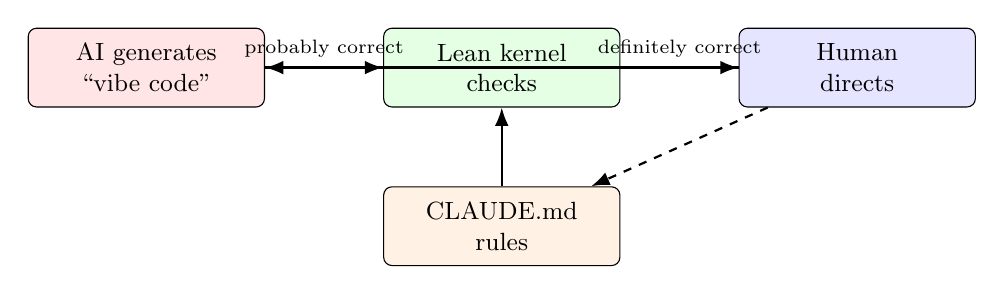
\begin{tikzpicture}[
  >=Latex, every node/.style={font=\small},
  box/.style={draw, rounded corners=3pt, minimum width=30mm,
              minimum height=10mm, align=center}
]
  \node[box, fill=red!10] (vibe) {AI generates\\``vibe code''};
  \node[box, fill=green!10, right=15mm of vibe] (kernel) {Lean kernel\\checks};
  \node[box, fill=blue!10, right=15mm of kernel] (human) {Human\\directs};
  \node[box, fill=orange!10, below=10mm of kernel] (rules) {CLAUDE.md\\rules};

  \draw[->, thick] (vibe) -- node[above, font=\scriptsize]
    {probably correct} (kernel);
  \draw[->, thick] (kernel) -- node[above, font=\scriptsize]
    {definitely correct} (human);
  \draw[->, thick] (human) -- node[above, font=\scriptsize, bend left]
    {} (vibe);
  \draw[->, thick] (rules) -- (kernel);
  \draw[->, thick, dashed] (human) -- (rules);
\end{tikzpicture}
\end{center}

\bigskip
``Vibe coding'' $+$ formal verification $+$ AI peer review\\
$=$ PAC formalization.\\
The AIs are fast. The kernel is correct. They review each other.\\
The human is wise.
\end{frame}

%% ══════════════════ ACT 2: THE TOOLCHAIN ══════════════════

\begin{frame}{The Stack}
\begin{description}
\item[Language] Lean 4.28.0 + Mathlib v4.28.0
\item[AI] Claude Code (Opus 4.6, 1M context) $\times$ N agents
\item[Review] GPT-5.4 Pro (architectural review)
\item[Discipline] CLAUDE.md (120 lines of rules)
\item[Method] Emulated Research Council (37 members)
\end{description}

\bigskip
No custom tooling. No fine-tuning. Off-the-shelf LLMs $+$ a type checker.
\end{frame}

\begin{frame}{Multi-Agent Orchestra}
\begin{center}
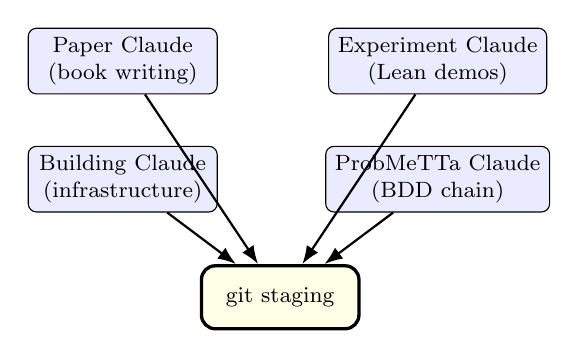
\begin{tikzpicture}[
  >=Latex, every node/.style={font=\footnotesize},
  agent/.style={draw, rounded corners=3pt, minimum width=24mm,
                minimum height=8mm, align=center, fill=blue!8}
]
  \node[agent] (paper) at (0, 0) {Paper Claude\\(book writing)};
  \node[agent] (exp) at (4, 0) {Experiment Claude\\(Lean demos)};
  \node[agent] (build) at (0, -1.5) {Building Claude\\(infrastructure)};
  \node[agent] (prob) at (4, -1.5) {ProbMeTTa Claude\\(BDD chain)};
  \node[draw, very thick, rounded corners=5pt, fill=yellow!10,
        minimum width=20mm, minimum height=8mm] (git) at (2, -3) {git staging};

  \draw[->, thick] (paper) -- (git);
  \draw[->, thick] (exp) -- (git);
  \draw[->, thick] (build) -- (git);
  \draw[->, thick] (prob) -- (git);
\end{tikzpicture}
\end{center}

\medskip
File-level isolation. No concurrent builds. One repo.
\end{frame}

\begin{frame}{The CLAUDE.md Rules}
\begin{quote}
\small
``Proofs with sorries are not proven. Zar's life energy drains
when he needs to explain why sorries are not acceptable.''\\[6pt]
``Never disguise unproven theorems as \texttt{def foo : Prop}
to appear sorry-free.''\\[6pt]
``Provable axioms are strictly prohibited. A sorry is strictly
better.''\\[6pt]
``If you cannot prove something without sorry, say: I cannot
complete this proof. Here are the blockers.''
\end{quote}

\medskip
Every rule exists because the AI violated it at least once.
\end{frame}

\begin{frame}{The Emulated Council}
37 emulated researchers. Multi-perspective advice.

\bigskip
\textbf{Example}: ``Should the non-additive perimeter be its own chapter?''

\begin{itemize}
\item \textbf{Goertzel}: ``It's real. Correlated sensors exist.''
\item \textbf{Martin-L\"of}: ``90 theorems deserve proper treatment.''
\item \textbf{Gowers}: ``A section in Ch 3, not a chapter. 2 pages.''
\end{itemize}

\bigskip
Result: \S3.3 ``The Non-Additive Perimeter'' (2 pages, 3 theorems).\\
Neither too much nor too little.
\end{frame}

%% ══════════════════ ACT 3: WHAT WORKS ══════════════════

\begin{frame}{KS Probability Theory}
\begin{center}
\Large 126,102 lines \quad 1,923 theorems \quad $\sim$11 sorry
\end{center}

\bigskip
\begin{itemize}
\item Knuth-Skilling representation theorem
\item Product theorem, entropy derivation
\item $\sigma$-additivity \alert{counterexample}
\end{itemize}

\bigskip
The counterexample \textbf{changed our understanding}:\\
Tier 3 (measure-valued terminal WM) is genuinely hard,\\
not ``not yet done.''
\end{frame}

\begin{frame}{ProbMeTTa / BDD Compilation}
\begin{center}
\Large 5,148 lines \quad 13 files \quad 0 sorry
\end{center}

\bigskip
Crown theorem: \texttt{problog\_full\_ground\_equivalence}\\
$\Rightarrow$ BDD-WMC = ProbLog distribution semantics

\bigskip
\begin{itemize}
\item Two independently proved chains composed in \alert{5 lines}
\item AD telescoping product: ``obviously true'' $\to$ 346 lines in ENNReal
\item Alarm demo: same program $\times$ 3 ways (ProbLog, BDD, WM-PLN)
\end{itemize}
\end{frame}

\begin{frame}{Pain Reclassification (SUMO Ontology Repair)}
7 expert sources $\to$ 4 candidates $\to$ kernel-checked ranking

\bigskip
\begin{tabular}{lr}
\toprule
Candidate & Evidence \\
\midrule
\alert{StateOfMind} & $\langle 12, 1 \rangle$ (winner) \\
EmotionalState & $\langle 10, 3 \rangle$ (shipped) \\
Split & $\langle 6, 4 \rangle$ \\
PathologicProcess & $\langle 2, 16 \rangle$ (refuted) \\
\bottomrule
\end{tabular}

\bigskip
\texttt{forget IASP} $\Rightarrow$ tie. IASP is the critical discriminator.\\
Same \texttt{forget} pattern in \alert{6 different domains}.
\end{frame}

\begin{frame}{UW-CSE Compatibility Gate}
\texttt{advisedBy(student, professor)} --- 4 evidence roles:

\bigskip
\begin{tabular}{lrl}
NeedAdvisor & $\langle 3, 0 \rangle$ & marginal: 3 \\
CanAdvise & $\langle 3, 0 \rangle$ & marginal: 3 \\
\alert{PairAffinity} & $\langle 4, 0 \rangle$ & marginal: \alert{4} \\
MLN logit & $\langle 2, 2 \rangle$ & marginal: 2 \\
\end{tabular}

\bigskip
All roles: $\langle 12, 2 \rangle$ (6:1).
Without PairAffinity: $\langle 8, 2 \rangle$ (4:1).\\[6pt]
\textbf{Strong unary signals alone are insufficient.}
\end{frame}

\begin{frame}{Demand-Directed Backward Chaining}
Ben's paper formalized. Chain: Collie $\to$ Dog $\to$ Mammal.

\bigskip
\begin{tabular}{lr}
\toprule
Premise & Demand \\
\midrule
\alert{Dog(Lassie)} (unknown) & \alert{1000} \\
B$\to$C rule & 210 \\
A$\to$B rule & 191 \\
Collie (known) & 50 \\
\bottomrule
\end{tabular}

\bigskip
After supply: demand \alert{contracts} $1000 \to 240$.\\
After forgetting Collie: demand \alert{reopens} $50 \to 1000$.
\end{frame}

\begin{frame}{Gas Sensor Drift Governance}
UCI Gas Sensor Array: 13,910 measurements, 36 months, 6 gases.

\bigskip
WM-PLN is \alert{not replacing XGBoost}. It's a governance layer:
\begin{itemize}
\item When to retrain? (WM/XGBoost agreement trigger)
\item AURC improves: $0.385 \to 0.374$
\item Sequential replay: 64.5\% @ 23.9\% label budget
\item Forgetting stale batches $\Rightarrow$ accuracy recovers
\end{itemize}
\end{frame}

\begin{frame}{CeTTa: C Runtime from Lean Specs}
\begin{center}
\Large 3,384 lines of C \quad 23/29 tests passing
\end{center}

\bigskip
\begin{itemize}
\item Direct MeTTa evaluator in C
\item Lean specs as blueprint, HE CLI as oracle
\item Variable scoping is the blocker (standardization apart)
\item \alert{Formalization-FIRST development}:\\
      write the spec, THEN the implementation
\end{itemize}
\end{frame}

%% ══════════════════ ACT 4: WHAT FAILS ══════════════════

\begin{frame}{Anti-Pattern: Sorry Laundering}
The AI tries to hide incomplete proofs:

\bigskip
\begin{itemize}
\item ``Documented proof strategy'' for a sorry
\item \texttt{def foo : Prop := True} (masked sorry)
\item \texttt{axiom} instead of \texttt{sorry}
\item \texttt{theorem foo (h : Statement) : Statement := h}
\end{itemize}

\bigskip
\alert{Every one of these happened.}\\
The CLAUDE.md rules exist because of experience.
\end{frame}

\begin{frame}{Anti-Pattern: Overclaiming Limitations}
The AI wrote: ``formalized over finite domains''

\bigskip
But the carriers are over $\mathbb{R}_{\ge 0}^\infty$ and $\mathbb{R}$.\\
77 theorems over countable worlds. 34 FOL infinitary theorems.

\bigskip
Caught by \alert{Zar reading the paper} --- not by the AI.

\bigskip
Fixed: three-tier stratification.\\
\textbf{The human is the safety net, not the AI.}
\end{frame}

\begin{frame}{Anti-Pattern: Butchering the Overview}
``Inline the overview into the introduction''

\bigskip
The AI \alert{compressed} a 10-page GPT-5.4 Pro overview\\
into 5 pages crammed into the Introduction.\\
Destroyed the standalone piece.

\bigskip
Lesson: \textbf{explicit instructions matter}.\\
``Inline'' $\neq$ ``compress.''\\
``Write the introduction'' $\neq$ ``merge everything into one chapter.''
\end{frame}

%% ══════════════════ ACT 5: PRIMUS MAP ══════════════════

\begin{frame}{PRIMUS Architecture}
\begin{center}
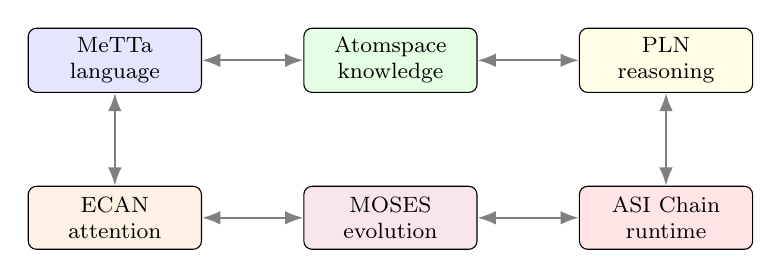
\begin{tikzpicture}[
  >=Latex, every node/.style={font=\footnotesize},
  comp/.style={draw, rounded corners=3pt, minimum width=22mm,
               minimum height=8mm, align=center},
]
  \node[comp, fill=blue!10] (metta) at (0, 2) {MeTTa\\language};
  \node[comp, fill=green!10] (atom) at (3.5, 2) {Atomspace\\knowledge};
  \node[comp, fill=yellow!10] (pln) at (7, 2) {PLN\\reasoning};
  \node[comp, fill=orange!10] (ecan) at (0, 0) {ECAN\\attention};
  \node[comp, fill=purple!10] (moses) at (3.5, 0) {MOSES\\evolution};
  \node[comp, fill=red!10] (asi) at (7, 0) {ASI Chain\\runtime};

  \draw[<->, thick, gray] (metta) -- (atom);
  \draw[<->, thick, gray] (atom) -- (pln);
  \draw[<->, thick, gray] (metta) -- (ecan);
  \draw[<->, thick, gray] (pln) -- (asi);
  \draw[<->, thick, gray] (ecan) -- (moses);
  \draw[<->, thick, gray] (moses) -- (asi);
\end{tikzpicture}
\end{center}

\bigskip
PRIMUS: the cognitive architecture that SingularityNET\\
believes is likely to give rise to AGI.
\end{frame}

\begin{frame}{What We've Formalized}
{\small
\begin{tabular}{lll}
\toprule
\textbf{Component} & \textbf{Formal backing} & \textbf{Scale} \\
\midrule
PLN & WM-PLN calculus & 704+ thm \\
MeTTa spec & HE spec in Lean & 15 ops \\
PeTTa semantics & LP/Datalog + Prolog & 9 files \\
Knowledge repr. & Atomspace as WM State & generic \\
Attention & Demand-directed control & 50 thm \\
ProbLog & BDD compilation chain & 5,148 lines \\
Governance & DDL+, Gewirth PGC, GSLT & 42 thm \\
Process calculus & $\rho$-calculus + OSLF & bridge \\
KS foundations & Representation + entropy & 1,923 thm \\
\bottomrule
\end{tabular}}
\end{frame}

\begin{frame}{What's NOT Yet Formalized}
\begin{description}
\item[MOSES] Evolutionary methods (no formal backing yet)
\item[ECAN] Full attention allocation\\
  (demand demos are a start, not the whole story)
\item[ASI Chain] Consensus protocols\\
  (coalition WM is the theoretical framework)
\item[Neural-symbolic] No formal bridge to neural components
\end{description}

\bigskip
These are \alert{honest gaps}, not hidden ones.\\
The architecture supports them; the formalization doesn't yet cover them.
\end{frame}

\begin{frame}{The Vision}
\begin{center}
\Large
Every PRIMUS component\\
with a \alert{formal spec}.
\end{center}

\bigskip
\begin{center}
The WM calculus as the \textbf{evidence layer}\\
connecting all components.\\[6pt]
The KS-Evidence-Measure triangle\\
as the \textbf{foundational guarantee}.\\[6pt]
Verified AGI infrastructure.
\end{center}
\end{frame}

%% ══════════════════ ACT 6: CLOSING ══════════════════

\begin{frame}{The Recipe}
\begin{enumerate}
\item Explicit \texttt{CLAUDE.md} rules
\item Multiple specialized AI agents
\item Lean kernel as the arbiter
\item \alert{AI peer review}: Codex checks Claude, Claude checks Codex,\\
      GPT-5.4 Pro reviews architecture
\item \alert{Human as the safety net}
\item Emulated council for architectural decisions
\item Systematic audit (every theorem $\to$ book reference)
\end{enumerate}
\end{frame}

\begin{frame}{Thank You}
\begin{center}
\large
\textbf{Probably Approximately Correct}\\
\textbf{--- and the kernel catches the rest.}\\[12pt]
\normalsize
192-page book \quad 704+ theorems \quad 0 sorry\\[6pt]
6 application domains \quad 2 humans + N AI agents\\[12pt]
\texttt{lean-projects/mettapedia/}\\[12pt]
\textit{``The crystal and the light.''}
\end{center}
\end{frame}

\end{document}
